
El ácido desoxirribonucléico, mejor conocido como ADN, o DNA en inglés (deoxyribonucleic acid), es la base de la biología molecular. Es esta biomolécula la que almacena la información genética de una célula, y es también a partir del procesamiento de esta molécula que surgen una infinidad de fenómenos de la biología. 

\section{Estructura del ADN}

AL igual que el resto de biomoléculas, el ADN se compone monómeros que, unidos, forman un polímero, el ADN. Los monómeros del ADN son los nucleótidos, y estos se componen de 3 compuestos claves.

\begin{figure}[H]
    \centering
    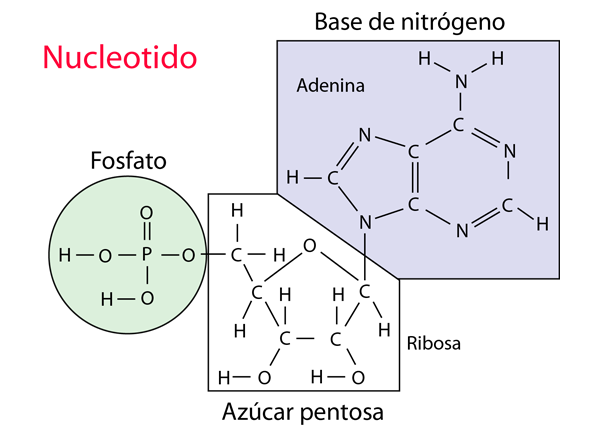
\includegraphics[width=0.75\linewidth]{images/estructura_de_un_nucleotido}
    \caption{Estructura general de un nucleótido}
    \label{fig:estructura_de_un_nucleotido}
\end{figure}

En primer lugar tenemos una base nitrogenada. Estas son compuestos orgánicos que cuentan con nitrógeno unido a ellos, y todos los organismos usan en su ADN las mismas 4 bases nitrogenadas: Adenina (A), timina (T), guanina (G) y citosina (C).

Luego de la base nitrogenada encontramos un carbohidrato, especificamente la 2-desoxi-D-ribosa, más comunmente acotada a desoxirribosa. A este carbohidrato (o azúcar) se le une una base nitrogenada en la posición 2'. 

Hasta este punto, la unión de una base nitrogenada con la ribosa se conoce como nucleósido. No es si no hasta que se une un grupo fosfato al extremo 5' del azúcar que podemos llamar a esta unión de moléculas un nucleótido, la unidad funcional del ADN.\cite{pinillabermudezBiologiaMolecular2019}

\section{Niveles de estructura del ADN}

\begin{figure}[H]
    \centering
    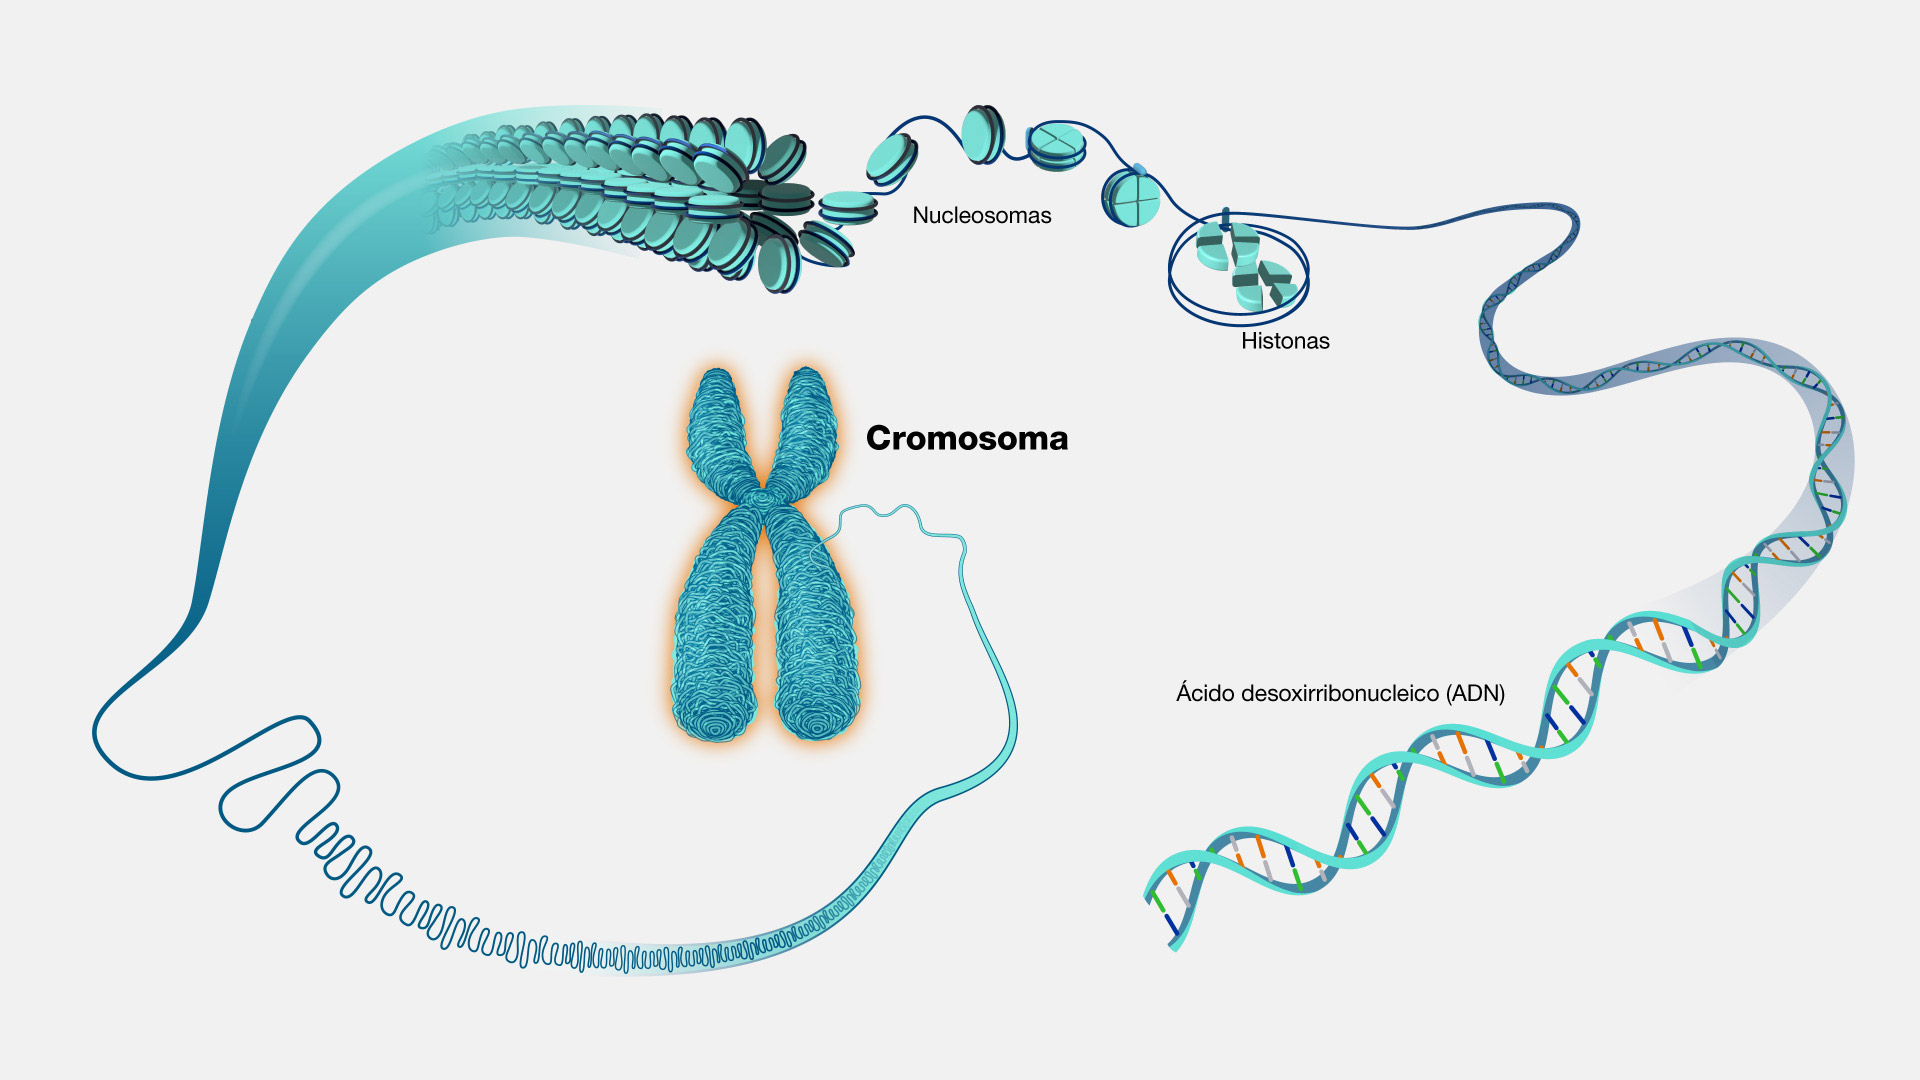
\includegraphics[width=\linewidth]{images/niveles_estructurales_del_adn}
    \caption{Niveles estructurales del ADN}
    \label{fig:niveles_estructurales_del_adn}
\end{figure}

Si bien los nucleótidos son la unidad estructural del ADN, no es la mera unión de estos lo que conforma a esta biomolécula, sino que se pueden identificar varias ``etapas'', los llamados niveles estructurales, a través de las cuales se va formando el ADN, y existen cuatro niveles estructurales en el ADN.

La estructura primaria, la más básica, se compone de la secuencia de nucleótidos en una hebra de ADN. Esto se refiere pues al orden específico en que una serie de nucleótidos estén ordenados.

Como segundo estructura secundaria tendríamos a la estructura que se forma al unir dos hebras de ADN, las cuales toman una forma de doble hélice. Estas hebras tienen dos características: son complementarias y antiparalelas.

La primer característica, la complementariedad, se refiere a que las bases nitrogenadas se unen de una manera específica entre ellas. Particularmente, toda adenina (A) se une siempre a una timina (T), y toda citosina (C) se une siempre a una guanina (G). 

La otra característica, el que las hebras sean antiparalelas, describe la orientación de los diferentes extremos de las hebras, los cuales son contrarios.

El nivel terciario consta del enrrollamiento de las hebras de ADN sobre unas proteínas llamadas histonas. Este enrrollamiento hace posible que el ADN se encuentre más compacto dentro de la célula, y sirve también como mecanismo de regulación génica (\autoref{sec:acetilación}).

Estas histonas pueden crear conjuntos entre sí llamados nucleosomas.

El último nivel, la estructura cuaternaria, un conjunto de nucleosomas se agregan entre sí para formar una nueva estructura, el selenoide. Esta estructura sirve para compactar aún más el ADN en los conocidos cromosomas. Este compactamiento es de gran relevancia durante la división celular.


\subsection{Histonas y nucleosomas}

Como se mencionó anteriormente, las histonas son proteínas sobre las cuales el ADN se enrrolla para compactarse. Estas proteínas se componen de 5 partes 

Las proteínas anteriormente mencionadas, las histonas, son proteínas que enrrollan el ADN, y se componen de 5 partes:

\begin{itemize}
    \item H1: Eslabón o linker
    \item H2A, H2B, H3, H4: Core
\end{itemize}

Como igualmente se mencionó antes, los nucelosomas son a su vez conjuntos de histonas que se agrupan entre sí.

\section{Modelos de replicación del ADN}

[PENDIENTE]

\section{Proceso de replicación} % En procariotas

Es el proceso en que el ADN de una célula se replica para preparase para la división celular. Este proceso se compone de 3 partes:

\begin{enumerate}
    \item Iniciación: Adherencia de proteínas al sitio de replicación (Ori)
    \item Elongación: Aquí trabaja la ADN polimerasa, moviéndose de 5' a 3'
    \item Terminación: Actividad de endo/exonucleasa
\end{enumerate}

\subsection{Componentes de la replicación}

\begin{itemize}
    \item Topoisomerasa: Esta va  por fuera del bucle. Desenrolla la cadena de ADN para que, posteriormente, la helicasa pueda romperla.
    \item Helicasa: Esta va por dentro del bucle. Rompe los enlaces de hidrógeno que unen a la cadena de ADN.
    \item Fragmentos de Okasaki: Se componen de ARN.
    \item Lugar de unión: Lugar donde las proteínas se unen a la hebra rezagada.
    \item Nucleotidos: Se transforman de ADN a ARN por acción de la proteína ADN ligasa. 
        \begin{itemize}
            \item Procariotas: 1000-2000 nucleótidos.
            \item Eucariotas: Menor cantidad de nucleótidos.
        \end{itemize}
        
    \item Cadenas
        \begin{itemize}
            \item Cadena principal: Trabaja de 3' a 5'
            \item Cadena rezagada: Trabaja de 5' a 3'. Aquí se aplican los fragmentos de Okazaki
        \end{itemize}
    \item Proteínas de unión: Se unen a los puntos de iniciación
    \item Proteínas de unión monocatenarias: Bloquean que se vuelva a enrollar la cadena
    \item ADNpolimerasa (ADNpol): Trabaja de 5' a 3'. Necesita de un grupo hidroxilo libre ($OH^{-}$).
    \item Primers, cebadores o iniciadores: Se colocan por actuar de la ARN primasa. Proporcionan el grupo hidroxilo libre ($OH^{-}$) que la ADNpol necesita. Se componen de 5-10 nucleotidos.
\end{itemize}

\subsection{Primera parte: Iniciación}

%Origen de replicación (Ori)

\subsection{Segunda parte: Elongación}



\subsection{Tercera parte: Terminación}



\section{Particularidades de la replicación eucariota}

Hay una serie de factores que influyen en que la replicación del ADN de células eucariotas sea algo más compleja. Estos son que el ADN de células eucariotas es más largo y se encuentra ``enrredado'' en proteínas llamadas histonas, las cuales al agregarse forman nucleosomas. Al darse la replicación del ADN, la hebra vieja se queda con los nucleosomas viejos y la hebra nueva se ``enrreda'' en histonas nuevas.


